E’ necessario fare una serie di premesse riguardo la scelta delle immagini da utilizzare nel programma, la quale risulta fondamentale per il corretto funzionamento dello stesso. Le immagini che verranno processate e successivamente utilizzate nel modello di training devono avere la stessa dimensione (non troppo piccola), in quanto dimensioni differenti porterebbero ad avere errori nel riconoscimento dell’iride e della pupilla. Le foto dell’occhio devono essere scattate frontalmente, poiché il programma non è sempre in grado di riconoscere l’iride se l’occhio è trasversale. E’ inoltre molto importante che l’occhio sia ben aperto, limitando il più possibile la presenza delle palpebre, in quanto risulterebbe falsata l’analisi di un segmento che le contiene anche solo parzialmente. 

\begin{figure}
  \centering
  \begin{subfigure}[b]{0.4\textwidth}
    \centering
    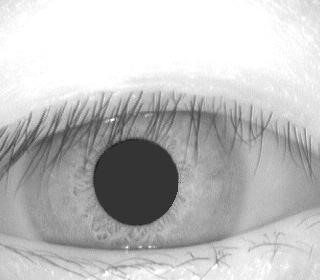
\includegraphics[width=\textwidth]{premesse_1}
    \caption{Immagine non ottimale}    
  \end{subfigure}
  \hfill
  \begin{subfigure}[b]{0.4\textwidth}
    \centering
    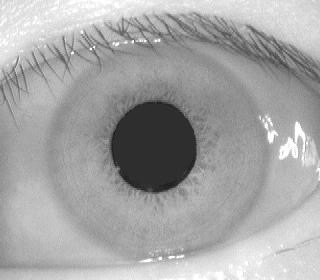
\includegraphics[width=\textwidth]{premesse_2}
    \caption{Immagine ottimale}       
  \end{subfigure}
  \caption{Esempi di immagini presenti nel dataset CASIA}
\end{figure}

Inoltre affinché un modello di machine learning produca risultati attendibili nel caso d’uso trattato, si dovrebbe utilizzare idealmente un elevato numero di immagini, equamente distribuite nelle classi di training. Un’ultima, importante premessa, va fatta riguardo il file di configurazione. In esso i parametri  sono settati appositamente per l’implementazione proposta. L’utilizzo di immagini differenti, in particolar modo di dimensioni diverse da quelle del dataset utilizzato in questo lavoro, comporta una dovuta modifica di alcuni di questi parametri, a carico dell’utente. Se non vengono modificati correttamente, i risultati dell’elaborazione potrebbero portare allo scarto di numerose immagini in seguito, ad esempio,  alla non corretta identificazione dei segmenti. 
